\section{T\={o}hoku Tsunami}
Our study focuses on quantifying ocean wave uncertainties associated with 
manning friction coefficient, 

The setting chosen for our experiment is the tsunami in the Pacific ocean 
that occurred in 11 March 2011. The 2011 earthquake off the Pacific coast of Tōhoku lasting approximately six minutes

%The earthquake, caused by 6 to 8 meters upthrust on a 180-km wide seabed at 60 km offshore from the east coast of Tōhoku, resulted in a major tsunami that brought destruction along the Pacific coastline of Japan's northern islands. Thousands of lives were lost when entire towns were devastated. The tsunami propagated throughout the Pacific Ocean region reaching the entire Pacific coast of North and South America from Alaska to Chile

\subsection{Computational Model}
Figure~\ref{fig:setup}(left) shows the topography of the considered domain.
Land topography is shown using while the bathymetry is shown using a lighter colormap.

During this tsunami, different gauges were installed to observed the surface elevation
The locations of theses gauges are shown in Figure~\ref{setup} .
The gauges are used in the inverse problem to infer the manning coefficients.

\begin{figure}[h]
\centering
\begin{tabular}{clc}
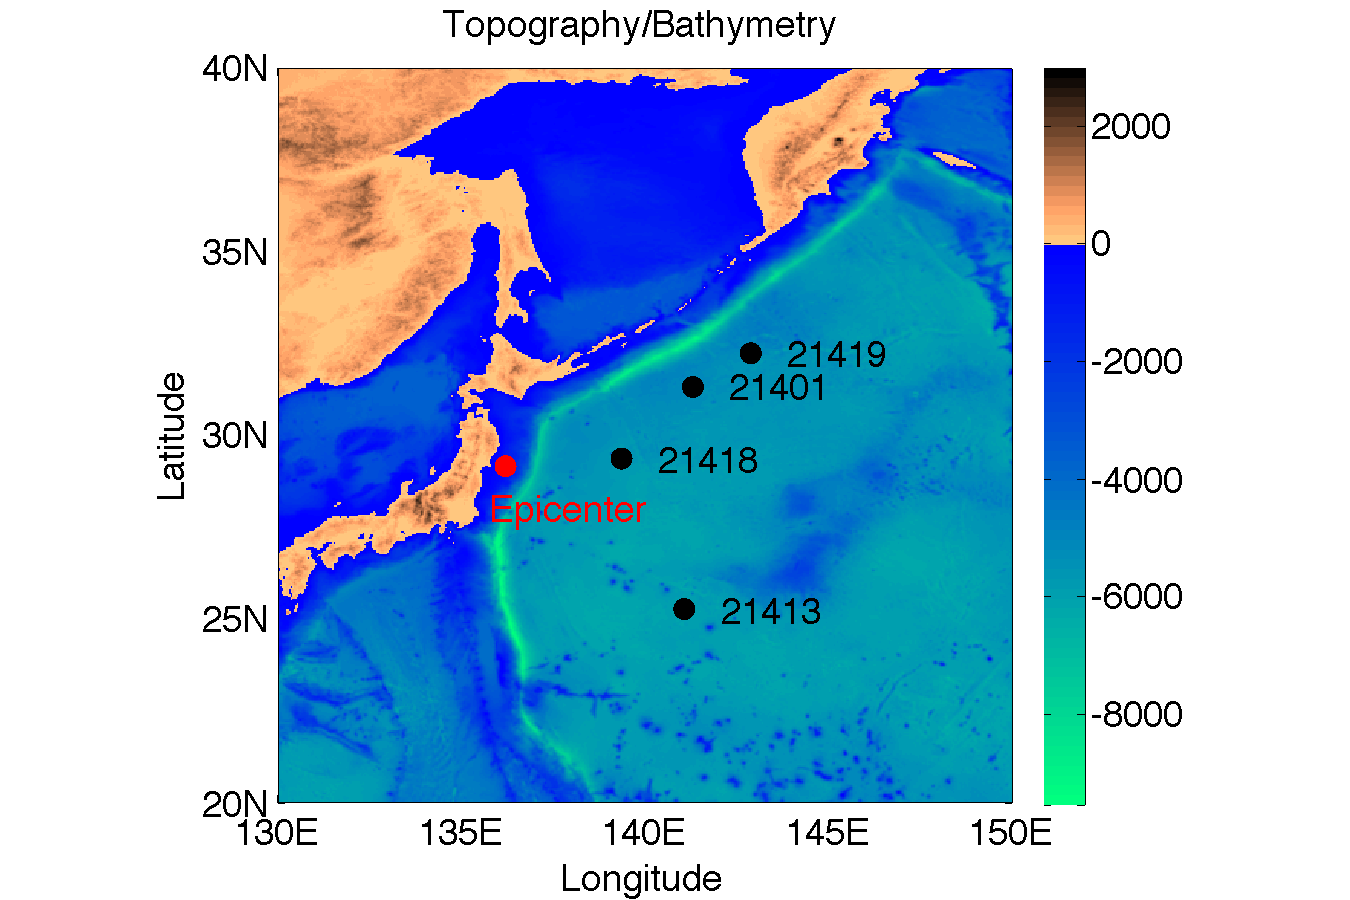
\includegraphics[width=0.45\textwidth]{../figures/topo.pdf}  &
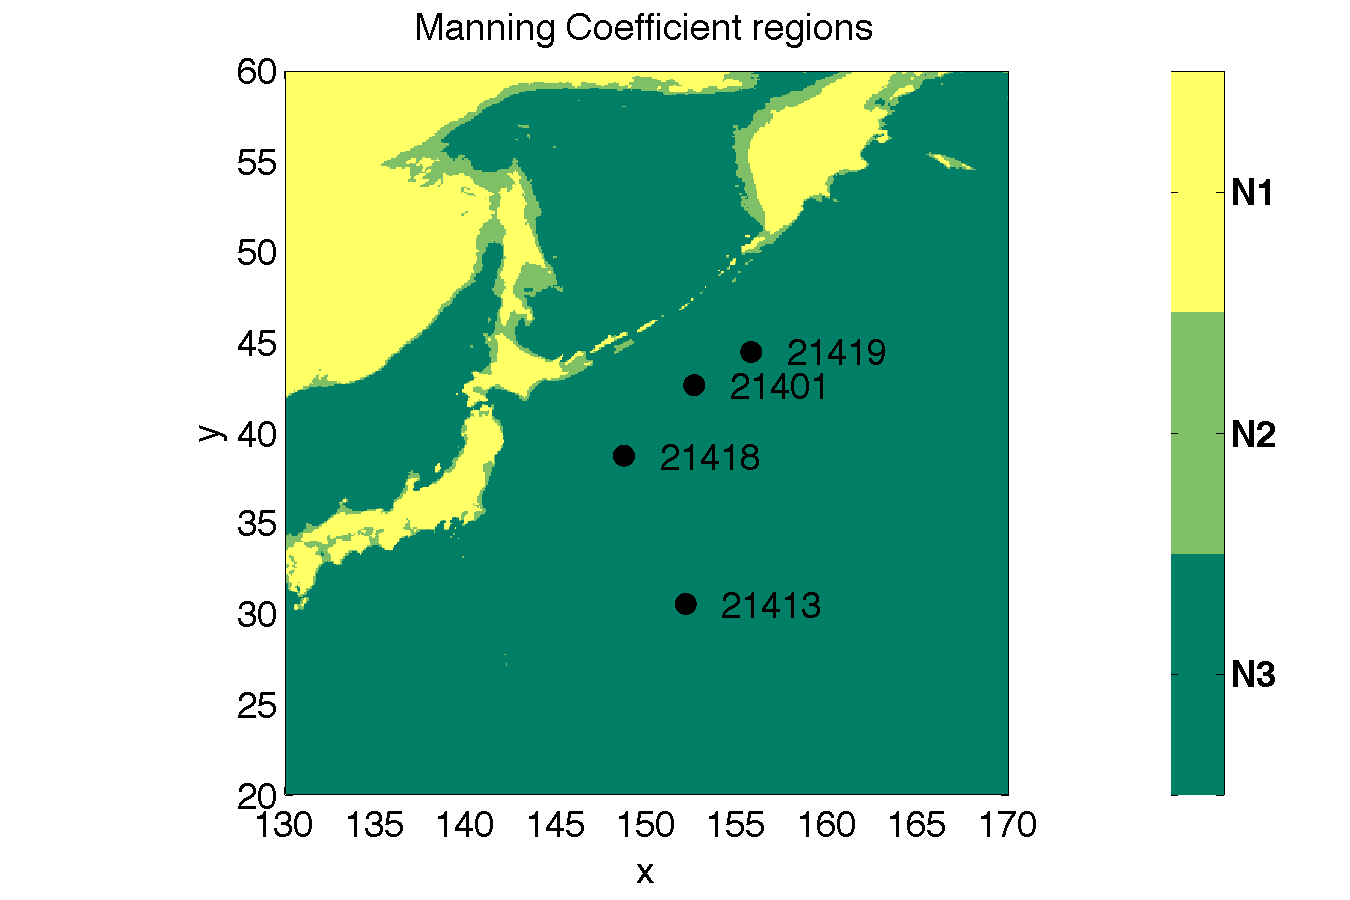
\includegraphics[width=0.45\textwidth]{../figures/coef.pdf} 
\label{setup}
\end{tabular}
\caption{Topography and gauge locations.}
\label{fig:setup}
\end{figure}